\documentclass[18pt]{beamer}
\usepackage[utf8]{inputenc} % for the umlauts
\usepackage{subfigure}
\usepackage{amssymb}% http://ctan.org/pkg/amssymb
\usepackage{pifont}% http://ctan.org/pkg/pifont
\newcommand{\cmark}{\ding{51}}%
\newcommand{\xmark}{\ding{55}}%
\newcommand{\correct}{\textcolor{green}{\cmark}}
\newcommand{\ncorrect}{\textcolor{red}{\xmark}}

\usepackage{tikz-uml}

\beamertemplatenavigationsymbolsempty
%% SLIDE FORMAT

% use 'beamerthemekit' for standard 4:3 ratio
% for widescreen slides (16:9), use 'beamerthemekitwide'

\usepackage{templates/beamerthemekit}
% \usepackage{templates/beamerthemekitwide}

\setcounter{tocdepth}{1}

%% TITLE PICTURE

% if a custom picture is to be used on the title page, copy it into the 'logos'
% directory, in the line below, replace 'mypicture' with the 
% filename (without extension) and uncomment the following line
% (picture proportions: 63 : 20 for standard, 169 : 40 for wide
% *.eps format if you use latex+dvips+ps2pdf, 
% *.jpg/*.png/*.pdf if you use pdflatex)

%\titleimage{mypicture}

%% TikZ INTEGRATION

% use these packages for PCM symbols and UML classes
 \usepackage{templates/tikzkit}
 \usepackage{templates/tikzuml}

% the presentation starts here

\usepackage{csquotes}
\usepackage{mathabx}
\usepackage{picture}
\usepackage[absolute,overlay]{textpos}
%\usepackage[texcoord,grid,gridunit=mm,gridcolor=red, subgridcolor=green]{eso-pic}
\setbeamercovered{invisible}
\setbeamertemplate{caption}{\raggedright\insertcaption\par}

\title[SWT1]{Softwaretechnik 1 - 4. Tutorium}
\subtitle{Tutorium 17}
\author{Felix Bachmann}
\date{25.06.2019}

\institute{KIT - Institut für Programmstrukturen und Datenorganisation (IPD)}
\begin{document}

% change the following line to "ngerman" for German style date and logos
\selectlanguage{ngerman}

%title page
\begin{frame}
\titlepage
\end{frame}

\begin{frame}{Was passiert heute?}
\tableofcontents
\end{frame}

\section{Feedback + Eval}
	\begin{frame}
	\frametitle{3. Übungsblatt Statistik}
	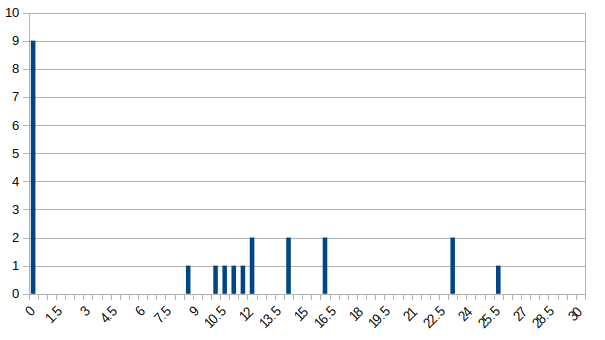
\includegraphics[scale=0.7]{./pics/tut3/statistics-ub3.png}
\end{frame}

\begin{frame}{Häufige Fehler: Blatt 3}
\begin{block}{Programmieraufgaben generell}
	\begin{itemize}
		\item wie letztes Mal gesagt \pause
		\item und das Mal davor \pause
		\item und das Mal davor \pause
		\item und das Mal davor \pause
		\item CheckStyle und Co.
		\pause
		\item nicht am JMJRST-Stil orientieren
		\begin{itemize}
			\item das können wir besser :)
		\end{itemize}
	\end{itemize}
\end{block} 

\begin{block}{Aufgabe 1 (\texttt{PluginManagement} + \texttt{PluginForJMJRST})}
\begin{itemize}
	\pause
	\item Plugins anhand \textbf{Klassen}namen vergleichen, 
	\begin{itemize}
		\item nicht \texttt{Object\#getName()}
		\item nicht \texttt{PluginForJMJRST\#getName()}
		\item z.B. \texttt{Object\#getSimpleName()}
	\end{itemize}
\end{itemize}
\end{block}
\end{frame}

\begin{frame}{Häufige Fehler: Blatt 3}
	\begin{block}{Aufgabe 2 (Instagrim Plug-In)}
	\begin{itemize}
		\pause
		\item Kommentarmenge komisch umgesetzt
		\begin{itemize}
			\item am einfachsten: String-Array
			\item dann aber keine magic numbers verwenden
			\begin{itemize}
				\item z.B. beim Ziehen der zufälligen Kommentare
			\end{itemize}
		\end{itemize}
		\pause
		\item Frame für \texttt{configure()}-Aufruf selbst gebaut
		\begin{itemize}
			\item kein Abzug solange kein Quatsch passiert und sinnvoll programmiert
			\item geht aber auch deutlich einfacher (siehe MuLö)
		\end{itemize}
	\end{itemize}
	\end{block}\pause

	\begin{block}{Aufgabe 3 (iMage-Bundle)}
	\begin{itemize}
	\item keine :D
	\end{itemize}
	\end{block}
\end{frame}

\begin{frame}{Häufige Fehler: Blatt 3}
\begin{block}{Aufgabe 4 (Aktivitätsdiagramm)}
	\begin{itemize}
	\pause 
	\item wie schon bei Anwendungsfalldiagramm
	\begin{itemize}
		\item Aktivitäten enthalten Verben
		\begin{itemize}
			\item es geht darum wer etwas tut
			\item \enquote{Startseite} ist keine Aktivität
			\item \enquote{Startseite anzeigen} schon
		\end{itemize}
	\end{itemize} \pause
	\item keine Partition verwendet/ falsche Syntax \pause
	\item Aktivitiäten = runde Ecken, Objekte = spitze Ecken \pause
	\item $\lbrack$\texttt{Bedingung}$\rbrack$ \pause
	\item Modellierung der Nutzerinteraktion
	\begin{itemize}
		\item z.B. \enquote{Klick} nachdem \enquote{Startseite anzeigen} vorbei? nicht sinnvoll
	\end{itemize}
	\end{itemize}
	\end{block}
\end{frame}

\begin{frame}{Häufige Fehler: Blatt 3}
	\begin{block}{Aufgabe 5 (Zustandsdiagramm)}
		\begin{itemize}
			\pause
			\item Übergänge von innerem parallelen Zustand \texttt{VxW} nach außen (\texttt{A}, \texttt{I})
			\begin{itemize}
				\item \texttt{VxW} ist auch nur ein Zustand
				\item auch wenn \enquote{innen drin} auch noch was passiert
				\item war in MuLö leider auch erst falsch
				\begin{itemize}
					\item deswegen bei einigen Korrekturen evtl. etwas Geschmiere an der Stelle, sorry!
				\end{itemize}
			\end{itemize}
		\end{itemize}
	\end{block}
\end{frame} 

\begin{frame}[fragile]{Häufige Fehler: Blatt 3}
	\begin{block}{Aufgabe 6 (Sequenzdiagramm)}
		\begin{itemize}
			\item allerlei Syntax-Kram
			\begin{itemize}
				\item Lebenslinien, Kästen, Doppelpunkte, Rückgabe-Notation
				\item asynchron vs. synchron (Pfeilspitzen wichtig) 
				\item kein Doppelpunkt bei \enquote{statischen Kästen} 
				\item \texttt{create} zeigt auf Kasten, nicht Lebenslinie/Steuerungsfokus
			\end{itemize}
			\pause
			\item Achtung: Steuerungsfokus ist zwar optional, erhöht aber stark die Lesbarkeit. In Klausur bitte verwenden. Bei Selbstaufrufen sonst problematisch, da Rückgabe ebenfalls optional. \pause
			\item Vorsicht bei Objekt-Zerstörung 
			\begin{itemize}
				\item \texttt{CameraCurve} vor Verwendeung zerstört
			\end{itemize}
		\end{itemize}
	\end{block}
	
\end{frame}

\begin{frame}[fragile]{Häufige Fehler: Blatt 3}
	\begin{block}{Aufgabe 7 (Substitutionsprinzip: Logger)}
		\begin{itemize}
			\pause
			\item Varianz war kein Problem
			\begin{itemize}
				\item getter: Kovarianz bei Rückgabetyp passt
				\item setter: Invarianter Parametertyp passt
			\end{itemize} \pause
			\item Problem war Verhalten, schwächere Nachbedingung \pause
			\item wurde oft zu schwammig formuliert
			\begin{itemize}
				\item oft sowas wie \enquote{Unterklasse tut nicht mehr dasselbe wie Oberklasse}
				\item aber das soll sie ja auch nicht, dann bräuchten wir kein Überschreiben von Methoden :)
			\end{itemize}
			\item bei solchen Aufgaben immer  aus Klient-Sicht anschauen
		\end{itemize}
	\end{block}
\end{frame}

\begin{frame}[fragile]{Häufige Fehler: Blatt 3}
	\begin{columns}
		\begin{column}{0.5\textwidth}
			\centering
			\begin{verbatim}
			O o = new O();
			o.m(x);
			
			o = new U(); 
			o.m(x);
			\end{verbatim}
		\end{column}%
		\begin{column}{0.5\textwidth}
			\begin{itemize}
				\item zweiter Aufruf \enquote{muss sich so verhalten wie} erster Aufruf
				\item Vorbedingung schwächer/gleich
				\item Nachbedingung stärker/gleich
			\end{itemize}
		\end{column}
	\end{columns}
	\pause
	\begin{itemize}
		\item \enquote{Unterklasse darf weniger verlangen, muss aber mehr leisten}
		\item (oder gleich viel)
		\item Hintergrund: Klient muss Unterklasse so benutzen können wie Oberklasse. Würde die Unterklasse bspw. mehr verlangen als Oberklasse müsste Klient wissen, dass er Unterklasse benutzt, um sie korrekt aufrufen zu können.
	\end{itemize}
\end{frame}


	\subsection{Feedback 4. Übungsblatt}
	\begin{frame}
		\frametitle{4. Übungsblatt Statistik}
		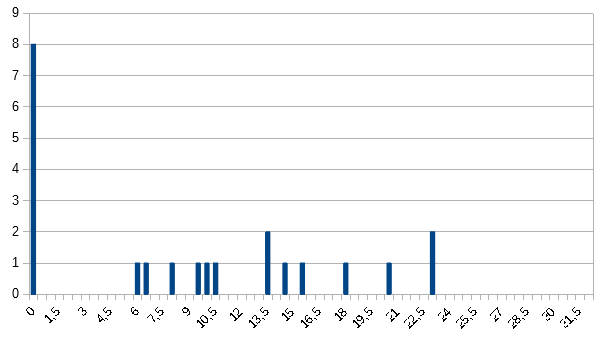
\includegraphics[scale=0.7]{./pics/tut4/statistics-ub4.png}
	\end{frame}
	
	\subsection{4. Übungsblatt - Fehler}
	\begin{frame}
		\frametitle{Häufige Fehler: Blatt 4}
		\begin{block}{Aufgabe 1: GUI für iMage}
			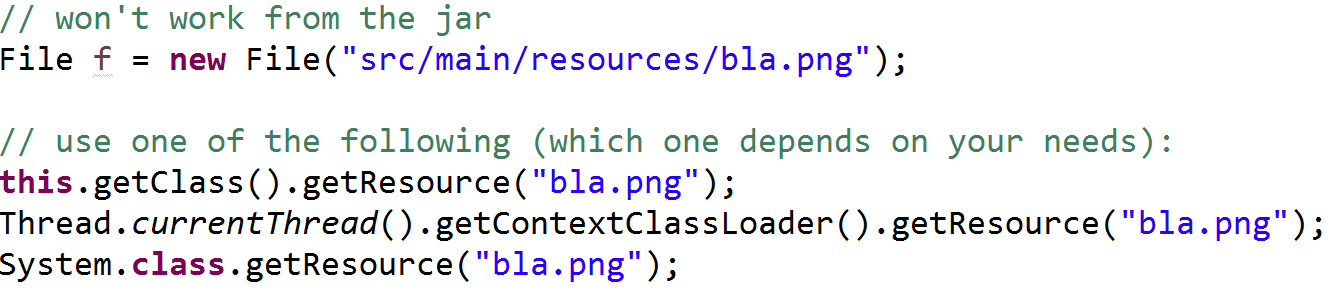
\includegraphics[scale=0.34]{./pics/tut5/file-resource.png}
			\begin{itemize}
				\pause 
				\item Gottklassen, wir wollen aber sinnvolle Objektorientierung \pause
				\item \texttt{SwingUtilities.invokeLater(e -> startGui())} benutzen
				\begin{itemize}
					\item ist thread safe (siehe nächstes Tut)
				\end{itemize} \pause
				\item nicht-navigierbare \texttt{JFileChooser} \pause
				\item Raw Types: \texttt{JComboBox} vs. \texttt{JComboBox<String>}
				\begin{itemize}
					\item ersteres nicht typsicher, müssen theoretisches jedes Mal \texttt{instanceof} aufrufen
				\end{itemize}
			\end{itemize}
		\end{block}
	\end{frame}

	\begin{frame}
		\frametitle{Häufige Fehler: Blatt 4}
		\begin{block}{Aufgabe 2: Aktivitätsdiagramm $\rightarrow$ Zustandsdiagramm}
			\pause
			\begin{itemize}
				\item \texttt{entry/}-Aktionen weggelassen, weil Zustand schon so heißt
				\begin{itemize}
					\item z.B. \enquote{StartseiteAnzeigen}
				\end{itemize} \pause
				\item \enquote{Brühvorgang beendet} fehlt, aber ok wenn anders sinnvoll modelliert
				\begin{itemize}
					\item sollte ja minimal sein
				\end{itemize}
			\end{itemize}
		\end{block}
		\pause 
		\begin{block}{Aufgabe 3: Geheimnisprinzip}
			\pause
			\begin{itemize}
				\item ist \textbf{nicht nur} private Attribute und \texttt{get(), set(x)} \pause
				\item verborgen wird immer \textbf{wie}, Interfaces sagen nur \textbf{was}
				\begin{itemize}
					\item auf \texttt{Closeable}-Objekt kann mittels \texttt{close()} Systemresource geschlossen werden
					\item unabhängig wie Zugriff auf Resource funktioniert
					\item einige impl. Klassen: \texttt{ZipFile, SSLSocket, AudioInputStream}
				\end{itemize}
			\end{itemize}
		\end{block}
	\end{frame}

	\begin{frame}
		\frametitle{Häufige Fehler: Blatt 4}
		\begin{block}{Aufgabe 4: Modul-Abhängigkeiten}
			\pause
			\begin{itemize}
				\item Systemgrenze \enquote{iMage} hat gefehlt \pause
				\item \texttt{commons-*}, \texttt{ojalgo}, \texttt{hamcrest-core} vergessen \pause
				\item Name sollten Modulnamen (intern) oder \texttt{artifactId} (extern) sein
				\begin{itemize}
					\item aber kein Abzug, solange erkennbar
				\end{itemize}
			\end{itemize}
		\end{block}
		\pause
		\begin{block}{Aufgabe 5: Entwurfsmuster in HDrize} \pause
			\begin{itemize}
				\item Abbildung Klassen zu Elementen aus VL-Muster fehlte
				\begin{itemize}
					\item z.B. \texttt{GrayScaleDecorater} ist \texttt{KonkreterDekorierer}
				\end{itemize}
			\end{itemize}
		\end{block}
	\end{frame}

\begin{frame}{Evaluation der Evaluation}
	leider nur 5 Teilnehmer??
	\centering
	\begin{table}
		\begin{tabular}{|c|c|}
			\hline 
			Gut & Schlecht/Verbesserungswürdig \\ 
			\hline
			Folien (3) & \\
			Beispiele und Code (3) & \\ 
			Erklärungen (2) & \\
			Tipps (2) & \\
			Aufgaben (2)&  zu viel Zeit für Aufgaben (2)\\ 
			&  Wahr/Falsch zu einfach (1)\\ 
			& nicht immer Lösungen auf Folie (1)\\
			& gleiche Beispiele wie in VL (1) \\
			& Bewertungen zu kurz (1)\\
			\hline 
		\end{tabular} 
	\end{table}
\end{frame}

\section{Recap}
	\subsection{Quiz(Adapter)}
	\begin{frame}
		\frametitle{Was bisher geschah..}
		\begin{itemize}
			\item haben uns Entkopplungmuster angeschaut \pause
			\linebreak $\implies$ Beobachter, Iterator, Adapter, Stellvertreter \pause
		\end{itemize}
		\begin{figure}
			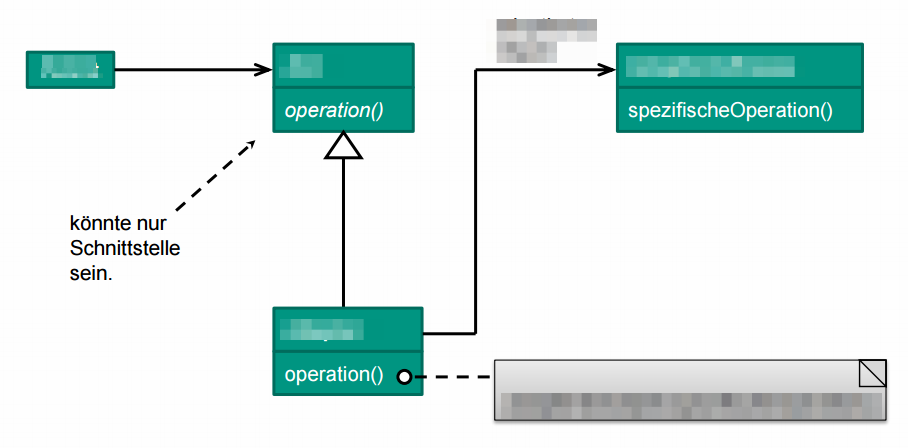
\includegraphics[scale=0.33]{./pics/tut4/adap-obj-mod.png}
		\end{figure}
		Welches Entwurfsmuster? \pause (Objekt-)Adapter
	\end{frame}
	
	\begin{frame}
		\frametitle{Was bisher geschah..}
		\begin{itemize}
			\item haben uns Entkopplungmuster angeschaut
			\linebreak $\implies$ Beobachter, Iterator, Adapter, Stellvertreter
		\end{itemize}
		\begin{figure}
			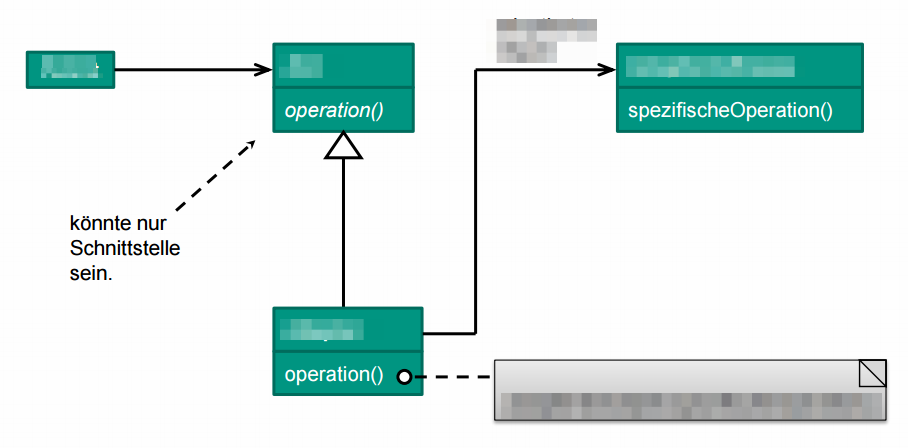
\includegraphics[scale=0.33]{./pics/tut4/adap-obj-mod.png}
		\end{figure}
		Welche Klassen?
	\end{frame}
	
	\begin{frame}
		\frametitle{Was bisher geschah..}
		\begin{itemize}
			\item haben uns Entkopplungmuster angeschaut
			\linebreak $\implies$ Beobachter, Iterator, Adapter, Stellvertreter
		\end{itemize}
		\begin{figure}
			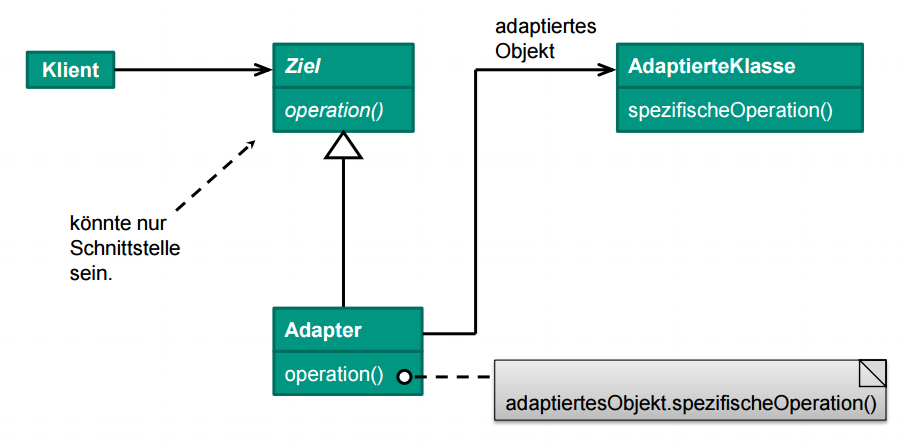
\includegraphics[scale=0.45]{./pics/tut3/adap-obj.png}
		\end{figure}
	\end{frame}
	
	\subsection{Quiz (Iterator)}
	\begin{frame}
		\frametitle{Was bisher geschah..}
		\begin{itemize}
			\item haben uns Entkopplungmuster angeschaut
			\linebreak $\implies$ Beobachter, Iterator, Adapter, Stellvertreter
		\end{itemize}
		\begin{figure}
			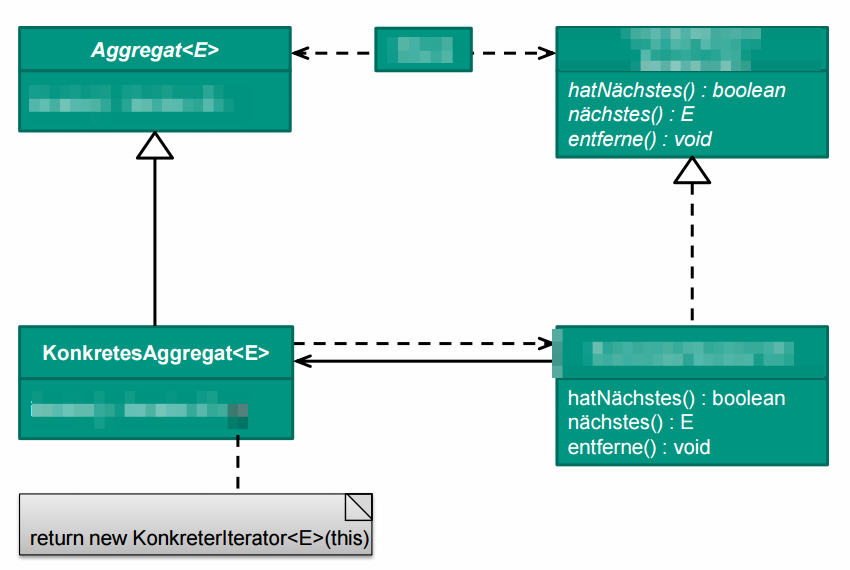
\includegraphics[scale=0.25]{./pics/tut4/iter-mod.png}
		\end{figure}
		Welches Entwurfsmuster? \pause Iterator
	\end{frame}
	
	\begin{frame}
		\frametitle{Was bisher geschah..}
		\begin{itemize}
			\item haben uns Entkopplungmuster angeschaut
			\linebreak $\implies$ Beobachter, Iterator, Adapter, Stellvertreter
		\end{itemize}
		\begin{figure}
			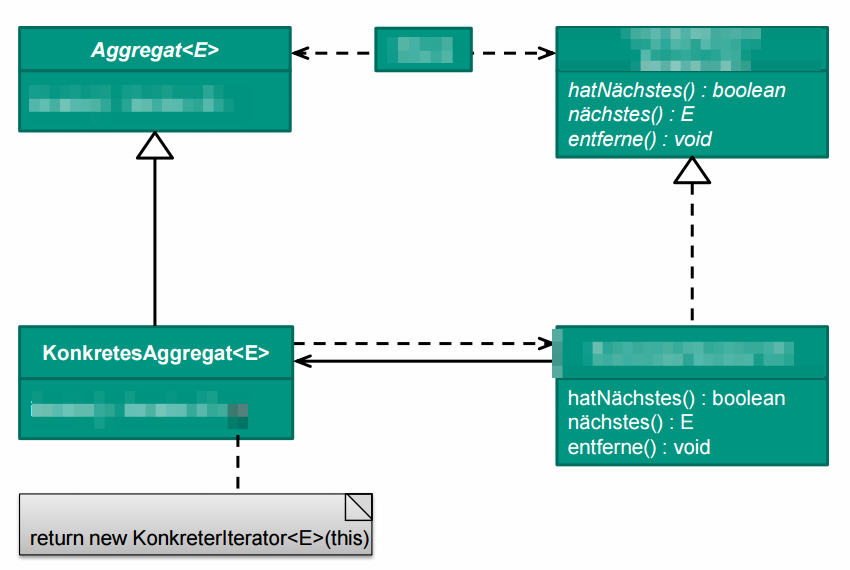
\includegraphics[scale=0.25]{./pics/tut4/iter-mod.png}
		\end{figure}
		Welche Klassen und Methoden?
	\end{frame}
	
	\begin{frame}
		\frametitle{Was bisher geschah..}
		\begin{itemize}
			\item haben uns Entkopplungmuster angeschaut
			\linebreak $\implies$ Beobachter, Iterator, Adapter, Stellvertreter
		\end{itemize}
		\begin{figure}
			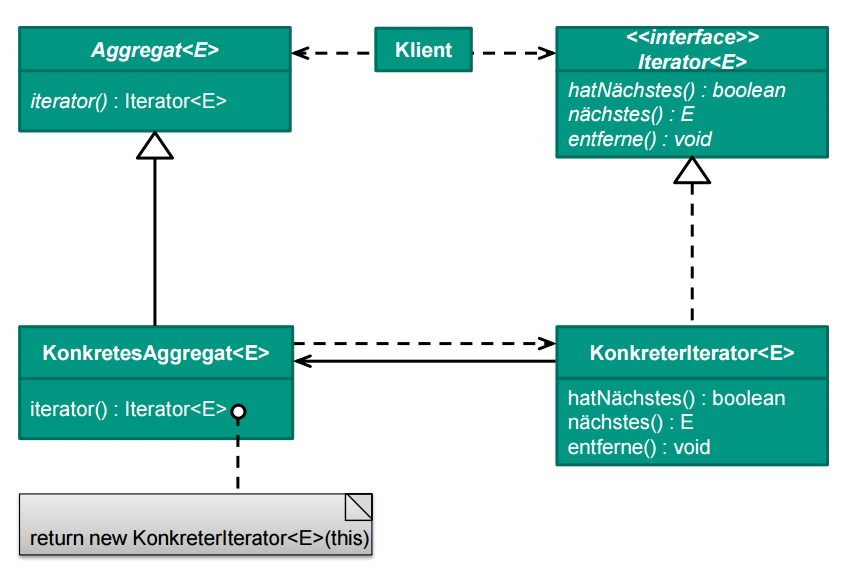
\includegraphics[scale=0.35]{./pics/tut3/iter.png}
		\end{figure}
	\end{frame}
	
	\subsection{Quiz(Beobachter)}
	
	\begin{frame}
		\frametitle{Was bisher geschah..}
		\begin{itemize}
			\item haben uns Entkopplungmuster angeschaut
			\linebreak $\implies$ Beobachter, Iterator, Adapter, Stellvertreter
		\end{itemize}
		\begin{figure}
			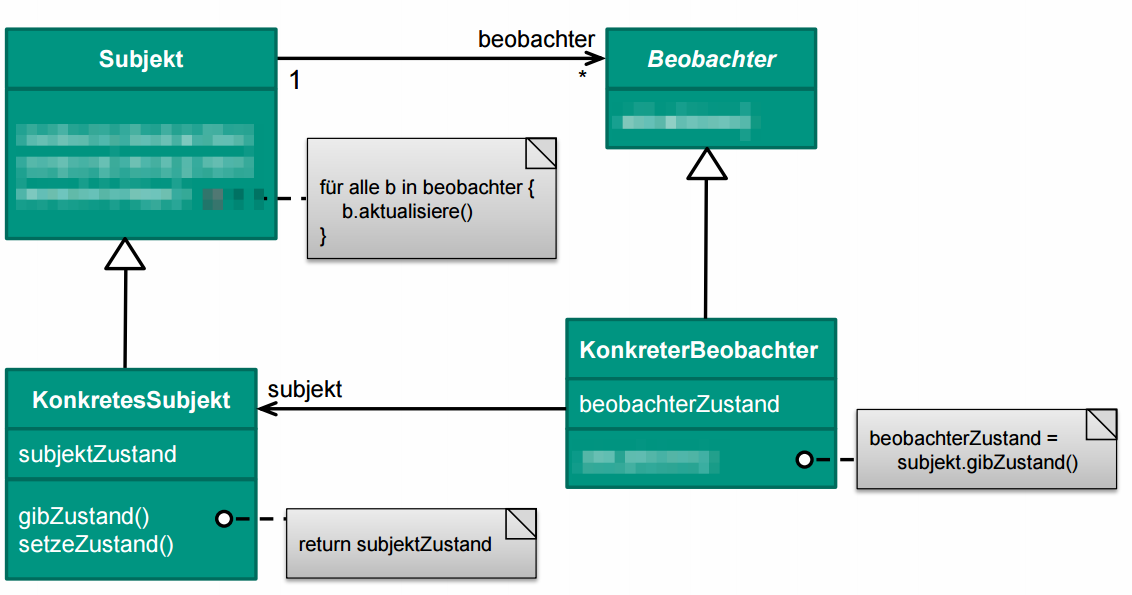
\includegraphics[scale=0.25]{./pics/tut4/obs-mod.png}
		\end{figure}
		\pause Ist wohl ein Beobachter :) \pause Methoden?
	\end{frame}
	
	\begin{frame}
		\frametitle{Was bisher geschah..}
		\begin{itemize}
			\item haben uns Entkopplungmuster angeschaut
			\linebreak $\implies$ Beobachter, Iterator, Adapter, Stellvertreter
		\end{itemize}
		\begin{figure}
			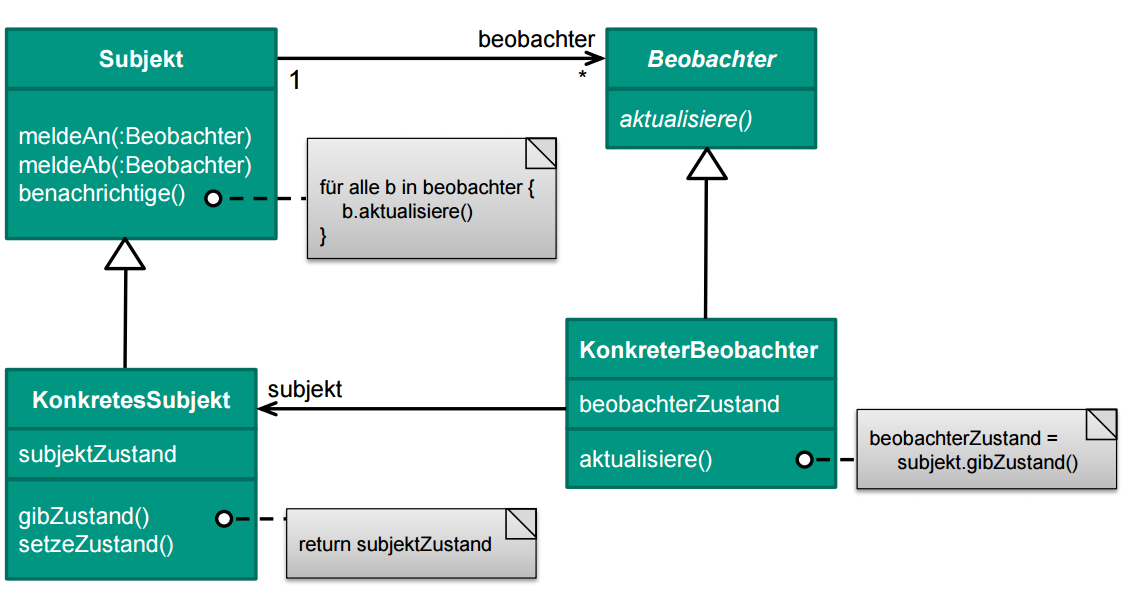
\includegraphics[scale=0.35]{./pics/tut3/obs.png}
		\end{figure}
	\end{frame}

\section{Vermittler}
	\begin{frame}
	\frametitle{Vermittler}
	
	\begin{block}{Problem}
		\begin{itemize}
			\item mehrere voneinander abhängige Objekte \linebreak \pause $\implies$ Zustände der Objekte von anderen Zuständen abhängig
		\end{itemize}
	\end{block}
	\pause
	\centering
	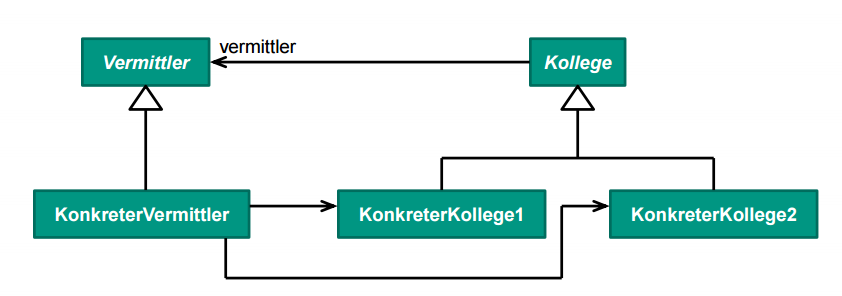
\includegraphics[scale=0.45]{./pics/tut3/med.png}
\end{frame}

\begin{frame}
	\frametitle{Vermittler}
	\centering
	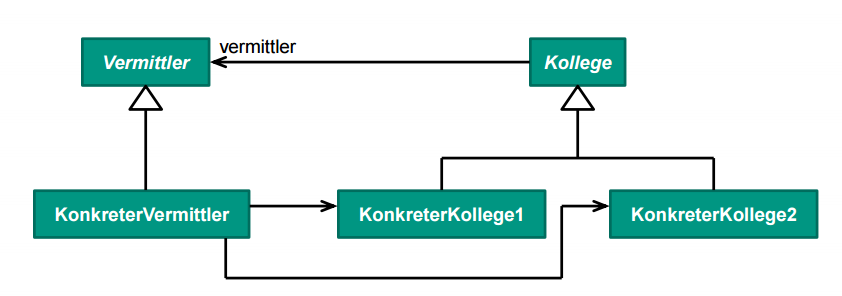
\includegraphics[scale=0.45]{./pics/tut3/med.png}
	\begin{block}{Entkopplung?}
	\begin{itemize}
		\pause 
		\item Kollegen kennen sich nicht direkt  \linebreak \pause $\implies$ Hinzufügen eines Kollegen erfordert keine Änderung der alten Kollegen
	\end{itemize}
	\end{block}
\end{frame}

\begin{frame}{Beobachter vs. Vermittler}
	\begin{itemize}
	\item wirken ähnlich
	\begin{itemize}
	\item ein Vermittler, viele Kollegen
	\item ein Subjekt, viele Beobachter
	\end{itemize}
	\end{itemize}
	\pause
	\begin{block}{Beobachter}
	Beobachter interessieren sich nicht füreinander. Nur für das Subjekt
	\end{block}
	\begin{block}{Vermittler}
	Kollegen interessieren sich füreinander, kommunizieren über den Vermittler miteinander.
	\end{block}
\end{frame}

\section{Aufgabe}
	\begin{frame}
	\frametitle{Klausuraufgabe (Hauptklausur SS 2012)}
	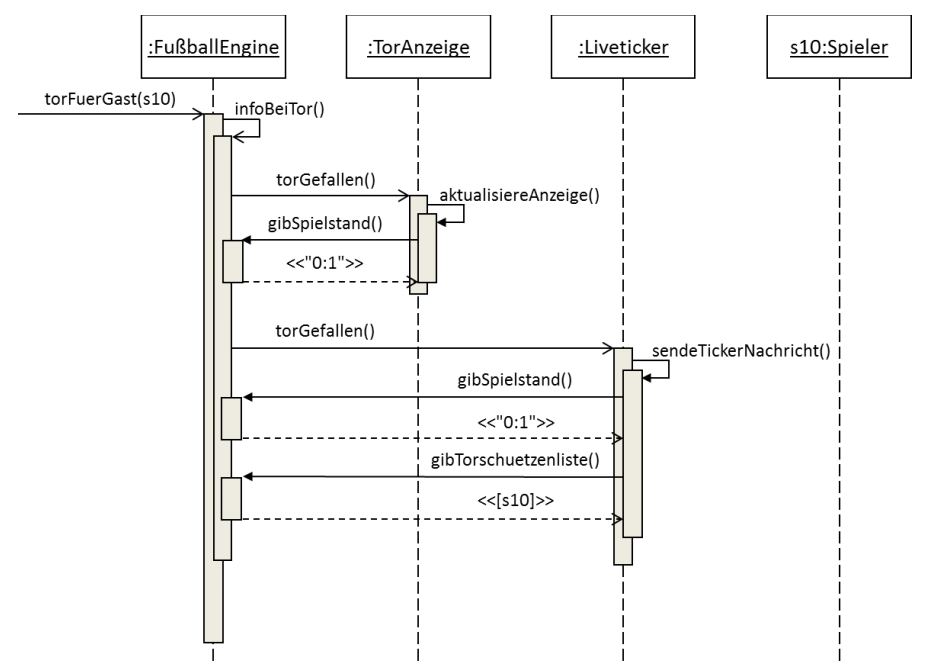
\includegraphics[scale=0.35]{./pics/tut3/obs-task.png}	
	\begin{block}{Aufgabe 1}
	Welches Entwurfsmuster erkennen Sie in diesem Diagramm? \pause
	Beobachter.
	\end{block}
\end{frame}

\begin{frame}
	\begin{small}
	Entwerfen Sie das folgende Klassendiagramm passend zu dem Sequenzdiagramm; es soll
	alle verwendeten Klassen und Methoden enthalten. Kennzeichnen Sie die Zugreifbarkeiten
	der Methoden mit den Symbolen +, -, \#; seien Sie dabei möglichst restriktiv. Verzichten
	Sie auf die Modellierung von Attributen. Kennzeichnen Sie die Elemente
	des Entwurfsmusters und deren Funktion.
	\end{small}
	\linebreak
	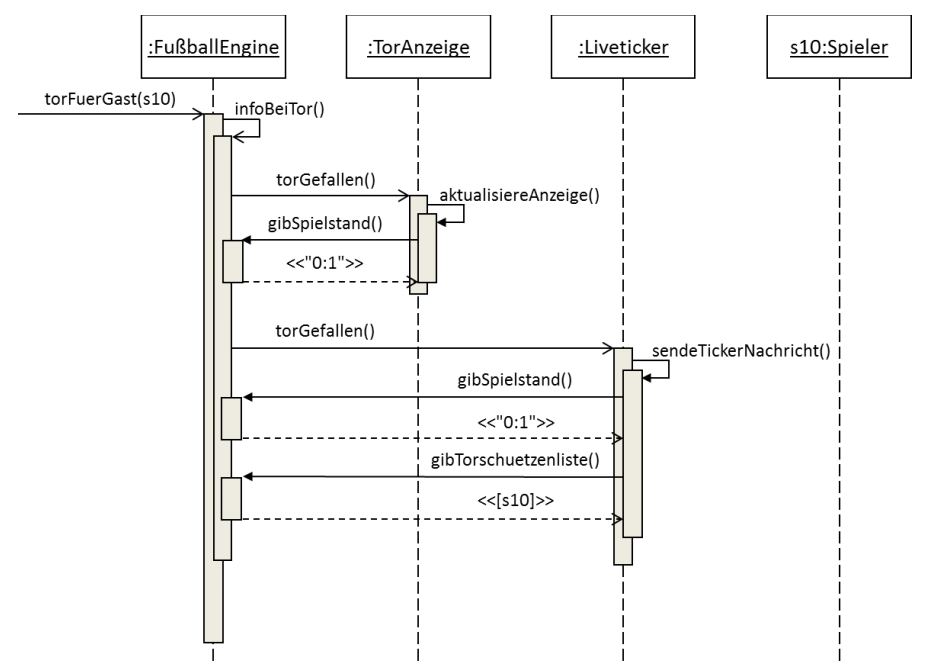
\includegraphics[scale=0.35]{./pics/tut3/obs-task.png}
\end{frame}

\begin{frame}
\frametitle{Musterlösung}
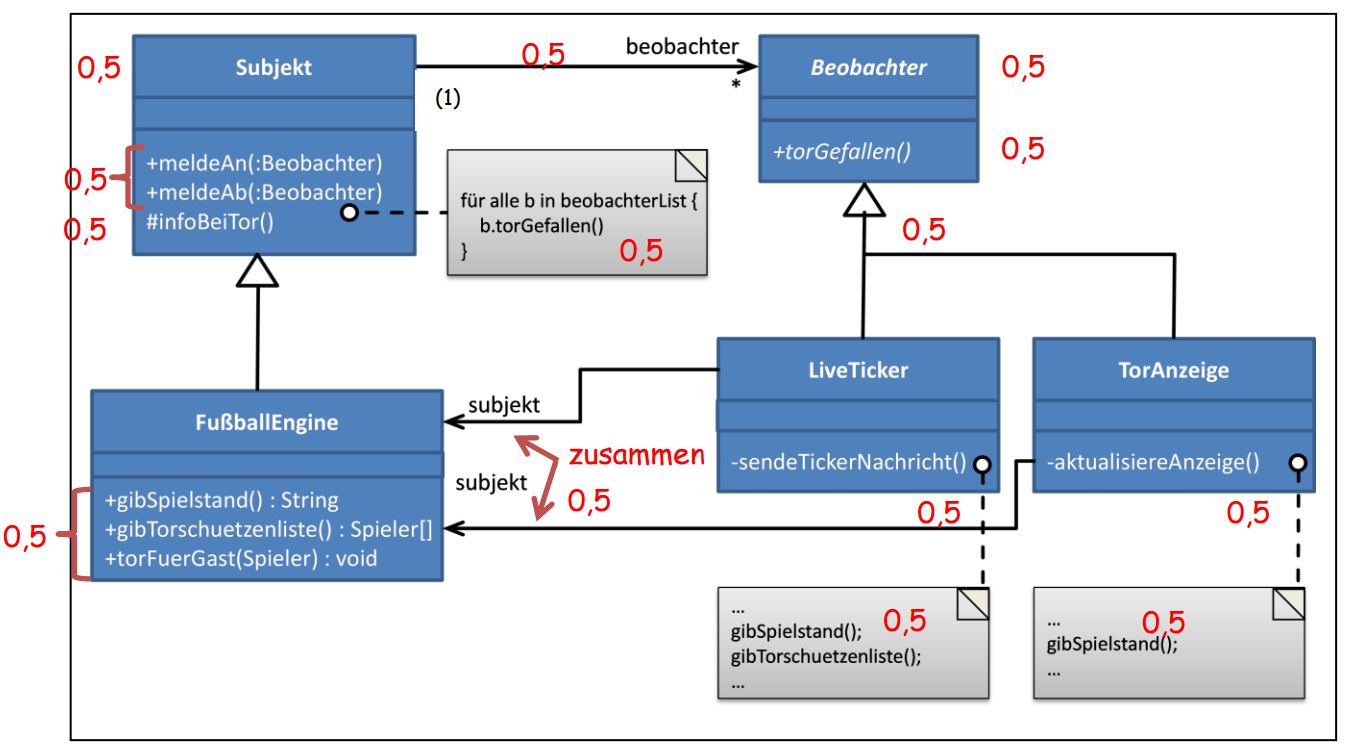
\includegraphics[scale=0.35]{./pics/tut3/obs-task-sol.png}
\end{frame}

\section{Rest Entwurfsmuster}
	\begin{frame}
		\frametitle{Kategorien der Entwurfsmuster}
		\begin{itemize}
			\item \textbf{Entkopplungs-Muster}
			\begin{itemize}
				\item Adapter \correct
				\item Beobachter \correct
				\item Iterator \correct
				\item Stellvertreter \correct
				\item Vermittler \correct
				\item (Brücke)
			\end{itemize}
			\item Varianten-Muster
			\item Zustandshandhabungs-Muster
			\item Steuerungs-Muster
			\item Bequemlichkeits-Muster
		\end{itemize}
	\end{frame}

	\begin{frame}
		\frametitle{Kategorien der Entwurfsmuster}
		\begin{itemize}
			\item Entkopplungs-Muster \correct
			\item \textbf{Varianten-Muster}
			\begin{itemize}
				\item (Abstrakte Fabrik)
				\item \textbf{Besucher}
				\item \textbf{Schablonenmethode}
				\item \textbf{Fabrikmethode}
				\item \textbf{Kompositum}
				\item Strategie \correct
				\item \textbf{Dekorierer}
			\end{itemize}
			\item Zustandshandhabungs-Muster
			\item Steuerungs-Muster
			\item Bequemlichkeits-Muster
		\end{itemize}
	\end{frame}
	

	
	\begin{frame}
		\frametitle{Varianten-Muster}
		\begin{block}{Übergeordnetes Ziel}
			\begin{itemize}
				\item Gemeinsamkeiten herausziehen und an einer Stelle beschreiben \pause
				\linebreak $\implies$ keine Wiederholung desselben Codes \pause
				\linebreak $\implies$ bessere Wartbarkeit/Erweiterbarkeit		
			\end{itemize}
		\end{block}
	\end{frame}

	\begin{frame}{Besucher}
		\begin{block}{Problem}
			\begin{itemize}
				\item Objekte sollen verarbeitet werden
				\item Verarbeitung der Objekte nicht als Methoden des Objektes
				\begin{itemize}
					\item Kapselung der Verarbeitung in \emph{Besucher}
					\item Besucher  \enquote{stattet Objekten einen Besuch ab} und verarbeitet sie dabei
				\end{itemize}
				\item Vorteile: gut neue Methoden hinzufügbar (durch neue Besucher)
			\end{itemize}
		\end{block}
	\end{frame}

	\begin{frame}{Besucher}
		\centering
		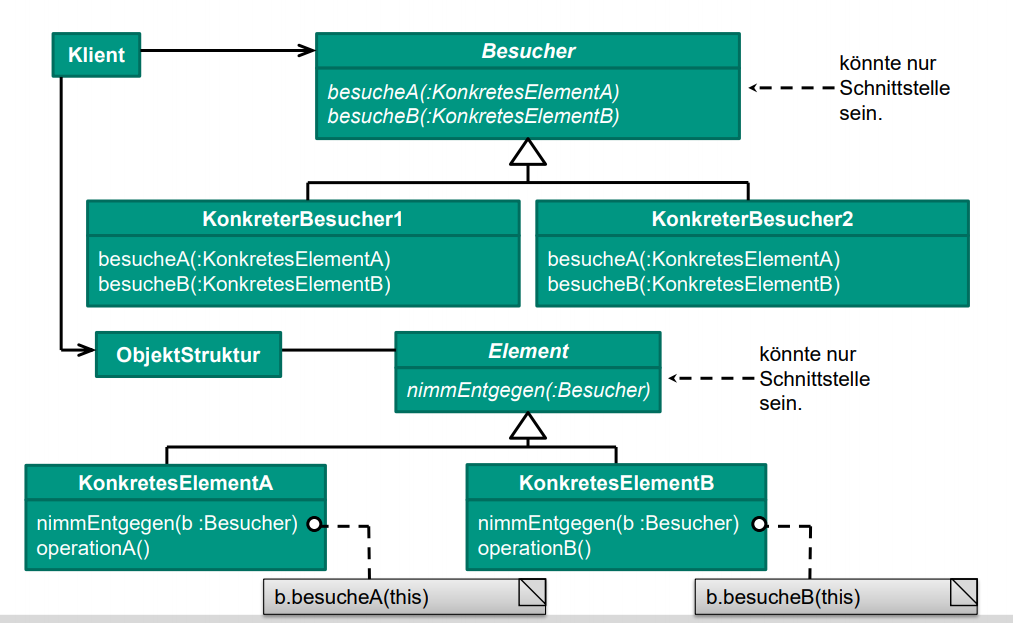
\includegraphics[scale=0.45]{pics/tut4/vis.png}
	\end{frame}

	\begin{frame}{Besucher}
	\begin{center}
		\begin{huge}
			 Code-Beispiel
		\end{huge}
	\end{center}
		\pause
		\begin{alertblock}{Achtung}
			\begin{itemize}
				\item Was ist ein großer Nachteil des Besucher-Musters?
				\item Womit wird die gute Erweiterbarkeit um Methoden erkauft? \pause
				\item schlecht um neue (Element-)Klassen erweiterbar!
			\end{itemize}
		\end{alertblock}
	\end{frame}

	\begin{frame}{Dekorierer}
		\begin{block}{Problem}
			\begin{itemize}
				\item dynamisch neue Funktionalität (=Methoden) zu Klasse hinzufügen
				\begin{itemize}
					\item aka \emph{dekorieren}
				\end{itemize}
				\item ohne Klasse zu ändern oder von ihr zu erben
				\item vermeidet unübersichtliche Vererbungshierarchien
				\begin{itemize}
					\item durch rekursives Dekorieren
				\end{itemize}
			\end{itemize}
		\end{block}
	\end{frame}

	\begin{frame}{Dekorierer}
		\begin{figure}
			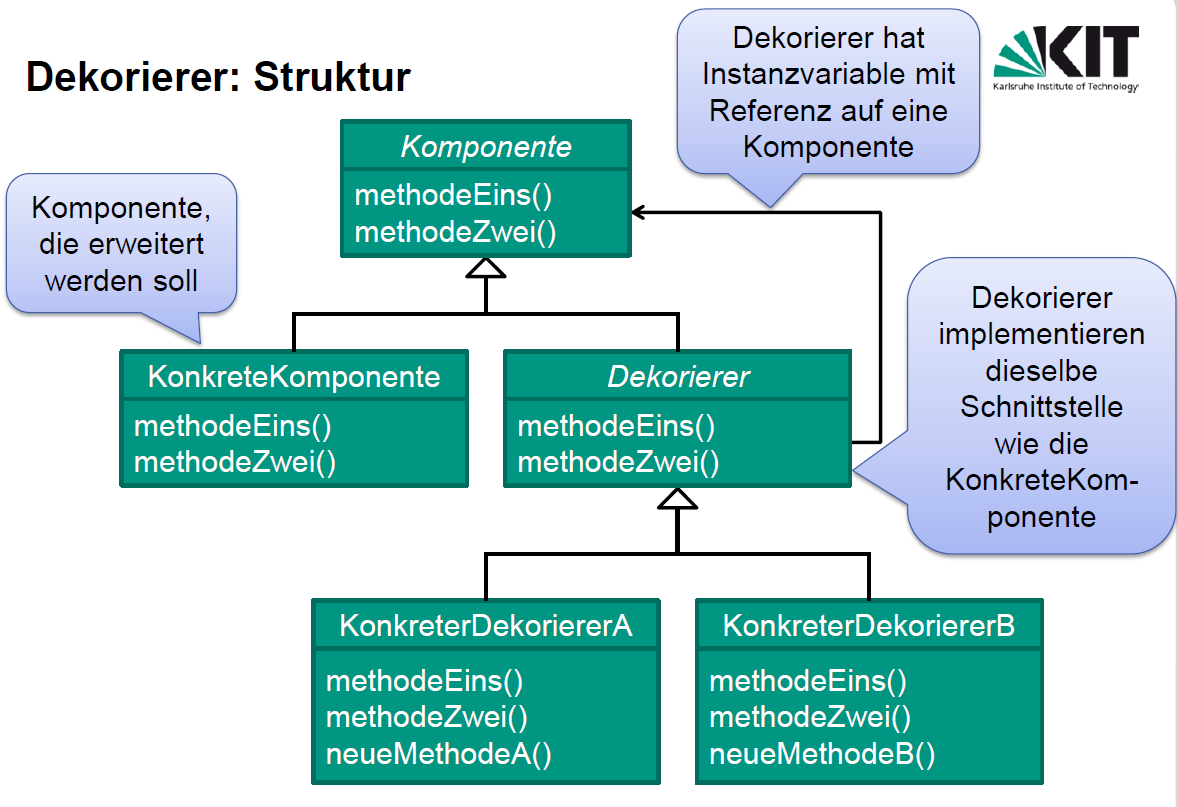
\includegraphics[scale=0.35]{./pics/tut4/decor.png}
		\end{figure}
	\end{frame}

	\begin{frame}[fragile]{Dekorierer}
		\begin{exampleblock}{Beispiel aus \texttt{java.io}}
			\begin{verbatim}
			// erstelle KonkreteKomponente
			FileInputStream fis = new FileInputStream("/objects.gz");
			// ab jetzt: dekorieren bis zum get no :)
			BufferedInputStream bis = new BufferedInputStream(fis);
			GzipInputStream gis     = new GzipInputStream(bis);
			ObjectInputStream ois   = new ObjectInputStream(gis);
			// Aufruf von neueMethode()
			SomeObject someObject   = (SomeObject) ois.readObject();
			// ...
			ois.close(); // delegiert an die "richtige Stelle" (fis)
			\end{verbatim}
		\end{exampleblock}
		\pause
		\begin{alertblock}{Ohne Dekorierer}
			z.B. Klasse \texttt{ObjectGzipBufferedFileInputStream} nötig
		\end{alertblock}
	\end{frame}

	\begin{frame}{Kompositum}
		\begin{block}{Problem}
			\begin{itemize}
				\item Bestandshierarchie modellieren
				\begin{itemize}
					\item zusammengesetzte und nicht-zusammengesetzte Objekte
					\item beide sollen einheitlich behandelt werden können
					\item leichtes Hinzufügen neuer Objekte
				\end{itemize}
			\end{itemize}
		\end{block}
	\end{frame}

	\begin{frame}{Kompositum}
		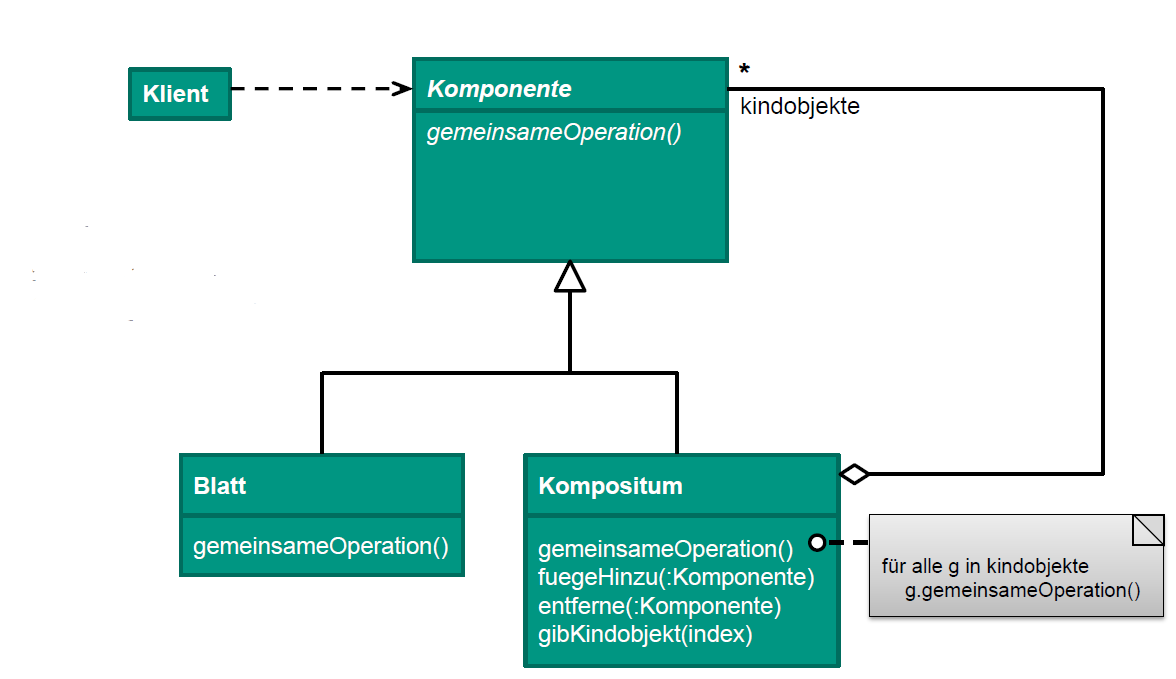
\includegraphics[scale=0.35]{./pics/tut4/comp.png}
		\pause
		Beispiel: \texttt{java.awt.Container\#add(Component comp)}
	\end{frame}

	\begin{frame}{Schablonenmethode}
		\begin{block}{Problem}
			\begin{itemize}
				\item eine Methode hat in allen Klassen, die sie implementieren, den gleichen Ablauf
				\item Teilschritte variieren aber
				\item nicht komplett in abstrakter Oberklasse implementierbar
			\end{itemize}
		\end{block}
	\end{frame}

	\begin{frame}{Schablonenmethode}
		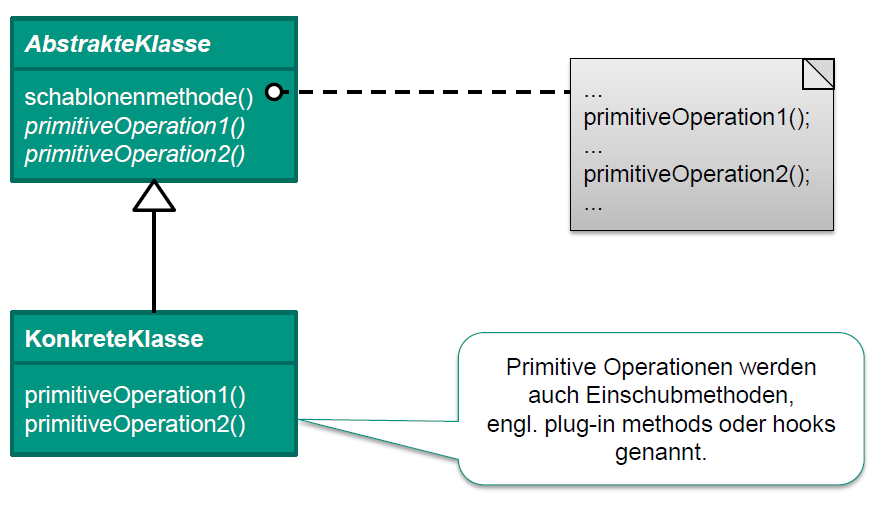
\includegraphics[scale=0.45]{./pics/tut4/schab.png}
	\end{frame}

	\begin{frame}{Schablonenmethode}
		\begin{huge}
			\begin{center}
				Code-Beispiel
			\end{center}
		\end{huge}
	\end{frame}

	\begin{frame}{Fabrikmethode}
		\begin{block}{Problem}
			\begin{itemize}
				\item Methode soll als Teil-Schritt ein Objekt erzeugen
				\item Unterklasse soll entscheiden, welches erzeugt wird
			\end{itemize}
		\end{block}
	\end{frame}

	\begin{frame}{Fabrikmethode}
		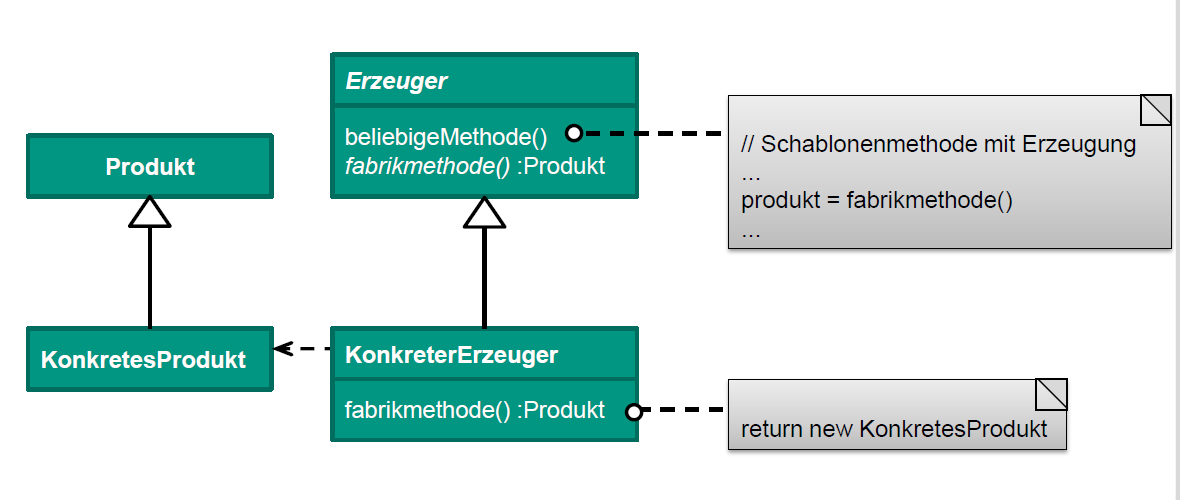
\includegraphics[scale=0.4]{./pics/tut4/fab.png}
	\end{frame}

	\begin{frame}{Ankreuzaufgaben aus Klausuren}
	Wahr oder falsch?
		\begin{itemize}
			\item Die Fabrikmethode sorgt dafür, dass nur eine einzige Instanz einer Klasse fabriziert wird. \pause \ncorrect \pause 
			\item Eine Schablonenmethode ist immer auch eine Fabrikmethode. \pause \ncorrect \pause
			\item Eine Komponente kann immer nur mit einem einzigen Dekorierer versehen werden. \pause \ncorrect
		\end{itemize}
	\end{frame}

	\begin{frame}{Kategorien der Entwurfsmuster}
		\begin{itemize}
			\item Entkopplungs-Muster \correct
			\item Varianten-Muster \correct
			\item \textbf{Zustandshandhabungs-Muster}
				\begin{itemize}
					\item \textbf{Einzelstück}
					\item (Fliegengewicht)
					\item \textbf{Memento} 
					\item (Prototyp) 
					\item (Zustand)
				\end{itemize}
			\item Steuerungs-Muster
			\item Bequemlichkeits-Muster
		\end{itemize}
	\end{frame}

	\begin{frame}
		\frametitle{Zustandshandhabungs-Muster}
		\begin{block}{Übergeordnetes Ziel}
			\begin{itemize}
				\item den Zustand eines Objektes beschreiben (wer hätt's gedacht? :D) \pause 
				\item aber unabhängig von dem Zweck des Objekts!
			\end{itemize}
		\end{block}
	\end{frame}

	\begin{frame}
		\frametitle{Einzelstück/Singleton}
		\begin{block}{Problem}
			\begin{itemize}
				\item von einer Klasse soll nur eine Instanz existieren
				\item Konstruktor könnte überall benutzt werden!
			\end{itemize}
		\end{block}
		\pause
		\centering
		\begin{figure}
			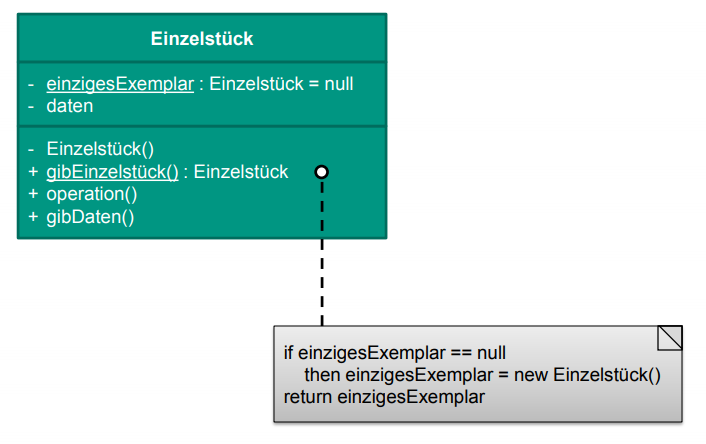
\includegraphics[scale=0.3]{./pics/tut4/singleton.png}
		\end{figure}
		\pause
		Aber warum nicht einfach statisch?\pause ~~ Unterklassenbildung möglich
	\end{frame}

	\begin{frame}
		\frametitle{Memento}
		\begin{block}{Problem}
			\begin{itemize}
				\item internen Zustand eines Objekts "'externalisieren"', um z.B. Zurücksetzen möglich zu machen \pause 
				\item ohne Kapselung zu verletzten
			\end{itemize}
		\end{block}
		\pause
		\centering
		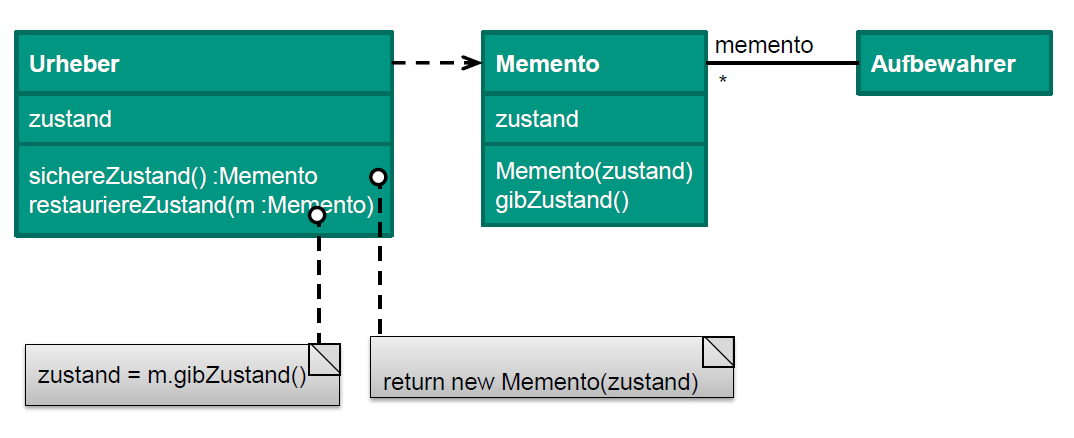
\includegraphics[scale=0.4]{./pics/tut4/mem.png}
	\end{frame}

	\begin{frame}
		\frametitle{Memento}
		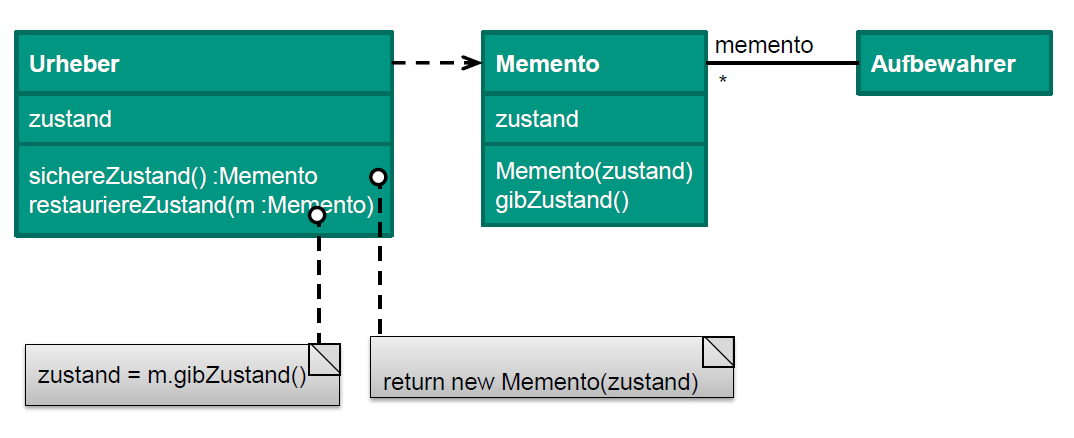
\includegraphics[scale=0.4]{./pics/tut4/mem.png}
		\begin{block}{Problem gelöst?}
			\begin{itemize}
				\pause
				\item Ja :)
				\begin{itemize}
					\pause
					\item Zustand durch Memento externalisiert \pause
					\item Kapselung nicht verletzt (kein direkter Zugriff auf Zustand)
					\item Nutzer ruft nur \texttt{sichereZustand()} auf und kriegt neuen Memento
				\end{itemize}
			\end{itemize}
		\end{block}
	\end{frame}

	\begin{frame}{Memento - Beispiel}
		\begin{figure}
			\centering
			\begin{tikzpicture}
			\pgfsetlayers{connections,main}
			\umlclass[x=-1.25,y=4,name=classname]
			{SuperMario}
			{
			 playerPos: Coordinate \\
			 coins: int\\
			 level: Level
		    }
			{
				save():Savegame\\
				load(s:Savegame)\\
				...
			}
			
			\umlclass[x=5,y=4, name=classname]
			{Savegame}
			{
				playerPos: Coordinate \\
				coins: int\\
				level: Level
	        }
			{
				$<<$create$>>$ Savegame(playerPos: Coordinate, \\~~~coins:int, level:Level)\\
				getPlayerPos(): Coordinate\\
				getCoins(): int\\
				getLevel(): Level
			}
			
			\umldep{SuperMario}{Savegame}
			\end{tikzpicture}
		\end{figure}
	\end{frame}

	\begin{frame}{Kategorien der Entwurfsmuster}
		\begin{itemize}
			\item Entkopplungs-Muster \correct
			\item Varianten-Muster \correct
			\item Zustandshandhabungs-Muster \correct
			\item \textbf{Steuerungs-Muster} 
				\begin{itemize}
					\item \textbf{Befehl}
					\item (master/worker)
				\end{itemize}
			\item Bequemlichkeits-Muster
		\end{itemize}
	\end{frame}
	
	\begin{frame}{Steuerungs-Muster}
		\begin{block}{Übergeordnetes Ziel}
			\begin{itemize}
				\item steuern den Kontrollfluss \pause 
				\linebreak $\implies$ zur richtigen Zeit richtige Methoden aufrufen
			\end{itemize}
		\end{block}
	\end{frame}

	\begin{frame}{Befehl}
		\begin{block}{Problem}
			\begin{itemize}
				\item Parametrisieren von Objekten mit einer auszuführenden Aktion \pause 
				\item komplexe Operationen aus primitiven Operationen aufbauen \pause
				\linebreak $\implies$ Befehl nicht als Methode, sondern als Klasse modellieren
			\end{itemize}
		\end{block}
		\pause
		\centering
		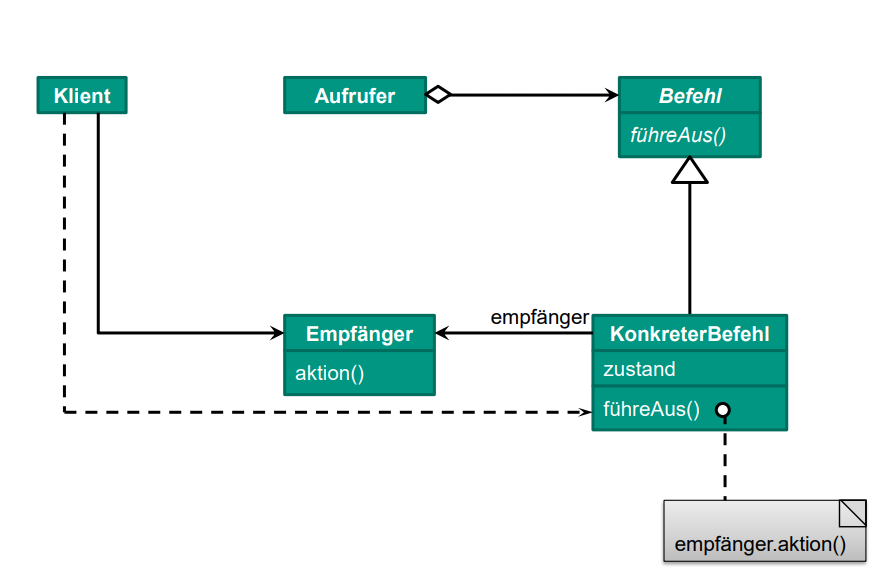
\includegraphics[scale=0.35]{./pics/tut4/command.png}
	\end{frame}

	\begin{frame}
		\frametitle{Befehl}
		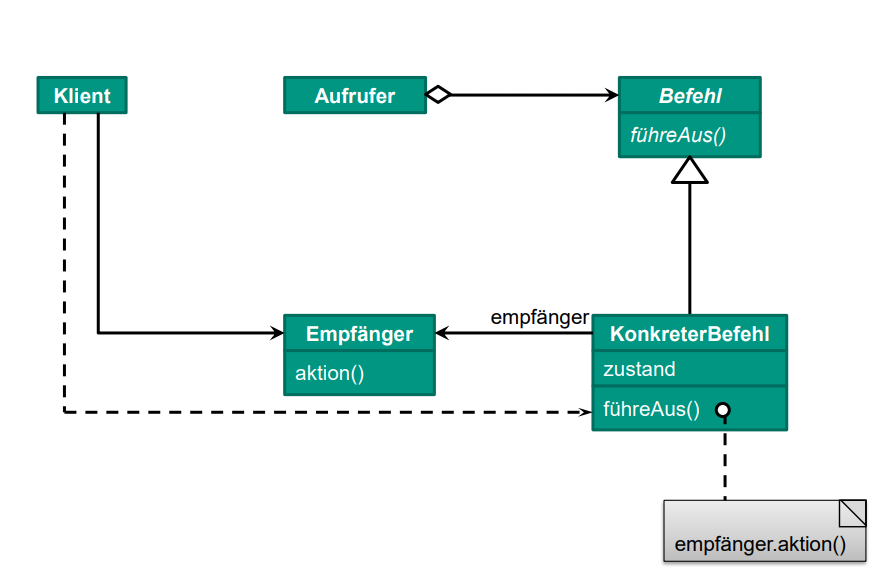
\includegraphics[scale=0.35]{./pics/tut4/command.png}
		\begin{block}{Was haben wir erreicht?}
			\begin{itemize}
				 \pause
				\item Austauschbarkeit: Befehle unabhängig vom Aufrufer, universell einsetzbar
			\end{itemize}
		\end{block}
	\end{frame}
	
	\begin{frame}
		\frametitle{Befehl}
		\centering \huge Code-Beispiel!
	\end{frame}

	\begin{frame}{Kategorien der Entwurfsmuster}
		\begin{itemize}
			\item Entkopplungs-Muster \correct
			\item Varianten-Muster \correct
			\item Zustandshandhabungs-Muster \correct
			\item Steuerungs-Muster \correct
			\item \textbf{Bequemlichkeits-Muster}
			\begin{itemize}
				\item (Bequemlichkeits-Klasse)
				\item (Bequemlichkeits-Methode)
				\item (Fassade)
				\item (Null-Objekt)
			\end{itemize}
		\end{itemize}
	\end{frame}

	\begin{frame}{Kategorien der Entwurfsmuster}
		\begin{itemize}
			\item Entkopplungs-Muster \correct
			\item Varianten-Muster \correct
			\item Zustandshandhabungs-Muster \correct
			\item Steuerungs-Muster \correct
			\item Bequemlichkeits-Muster \correct :)
		\end{itemize}
	\end{frame}
	
	\begin{frame}
		\frametitle{Ankreuzaufgaben aus Klausuren}
		Wahr oder falsch?
		\begin{itemize}
			\item Bei dem Entwurfsmuster Befehl kennt der Empfänger den Befehl nicht, jedoch der Befehl den Empfänger. \pause \correct \pause
			\item Ein Aufbewahrer im Entwurfsmuster Memento kann beliebig viele Mementos verwalten. Für die Restauration im Falle eines Reset ist er allerdings nicht verantwortlich. \pause \correct
		\end{itemize}
	\end{frame}
	
	\begin{frame}{Weitere Beispiele aus Java-Bibliotheken}
			\begin{center}
				\url{https://stackoverflow.com/questions/1673841/examples-of-gof-design-patterns-in-javas-core-libraries/}
			\end{center}
	\end{frame}
	
	\begin{frame}
		\frametitle{Für die Klausur}
		\begin{itemize}
			\item Entwurfsmuster kommen sehr sehr sehr wahrscheinlich dran \pause 
			\item Kategorien helfen beim Lernen \pause
			\item jedes Entwurfsmuster erfüllt einen bestimmten Zweck 
			\begin{itemize}
				\item nicht nur die Klassen und Methoden auswendig lernen, sondern das Prinzip verstehen
			\end{itemize}
		\end{itemize}
	\end{frame}


	
\section{Tipps}
	\subsection{Tipps}
	\begin{frame}
		\frametitle{Tipps - 5. Übungsblatt}
			\begin{exampleblock}{Aufgabe 1: Architekturstile} 
				\begin{itemize}
					\item MVC als Schichtenmodell
					\item wurde mal in der Vorlesung angesprochen, wie man das machen kann
				\end{itemize}
			\end{exampleblock}
			\pause
			\begin{exampleblock}{Aufgabe 2: Entwurfsmuster in API finden} 
				\begin{itemize}
					\item keine Tipps, sonst zu einfach :)
				\end{itemize}
			\end{exampleblock}
			\pause
			\begin{exampleblock}{Aufgabe 3: Iterator und Besucher selbst schreiben}
				\begin{itemize}
					\item Tiefensuche und Breitensuche als Iterator schreiben
					\item Verarbeitung der Baum-Elemente über Besucher realisieren
					\item Testfälle diesmal verpflichtend
				\end{itemize}
			\end{exampleblock}
	\end{frame}

	\begin{frame}
		\frametitle{Tipps - 5. Übungsblatt}
			\begin{exampleblock}{Aufgabe 4: Code zu Klassendiagramm}
				\begin{itemize}
					\item für Umsetzung von \texttt{Set}, \texttt{Map} nochmal Assoziationen anschauen
				\end{itemize}
			\end{exampleblock}
			\pause
			\begin{exampleblock}{Aufgabe 5: Zustandsautomat implementieren}
				\begin{itemize}
					\item Tests wieder verpflichtend
					\item Folien zu Zustands-Muster arg knapp
					\item die im Implementierungskapitel sind deutlich ausführlicher
				\end{itemize}
			\end{exampleblock}
			\pause
			\begin{exampleblock}{Aufgabe 6: Git}
				\begin{itemize}
					\item \texttt{git merge} vs. \texttt{git rebase}
					\item \enquote{Merge preserves history whereas rebase rewrites it.}
					\item \url{https://learngitbranching.js.org/}
					\begin{itemize}
						\item interaktives, visuelles Tool zum tieferen Verständnis von git
						\item merge und rebase: Level 1.3 und 1.4
					\end{itemize}
 				\end{itemize}
			\end{exampleblock}
	\end{frame}
	
	\subsection{Abgabe}
	\begin{frame}
		\frametitle{Das vorletzte Blatt..}
		\begin{alertblock}{Abgabe}
			\begin{itemize}
				\item Deadline am 03.07.19 um 12:00
				\item Aufgaben 1,2,4,6 handschriftlich
			\end{itemize}
		\end{alertblock}
	\end{frame}
		
	\begin{frame}
		\frametitle{Bis dann! (dann  := 09.07.19)}
		\begin{itemize}
			\item Servicehinweis: Steam Summer Sale ab heute :)
		\end{itemize}
		\centering
		
\includegraphics[scale=0.4]{./pics/tut4/steam.jpg}
		%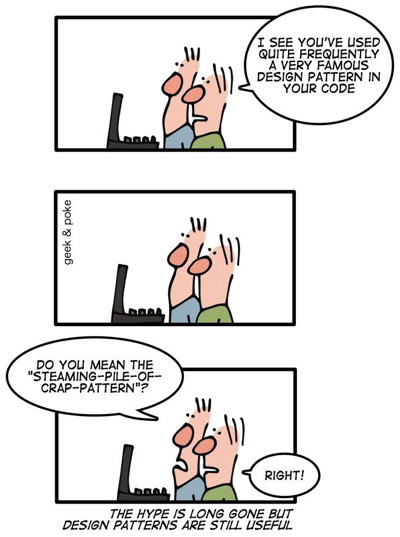
\includegraphics[scale=0.4]{./comics/patterns.jpg}
	\end{frame}

\end{document}